\newcommand{\docNome}{Piano di Progetto}                          % NOME DEL DOCUMENTO
\newcommand{\docVersione}{0.0.5}                 % INSERIRE VERSIONE IN FORMATO x.y.z
\newcommand{\docStatus}{in lavorazione}          % AGGIORNARE SOLO QUANDO APPROVATO
\newcommand{\docUso}{Esterno}                           % INTERNO O ESTERNO
\newcommand{\docDestinatari}{
      Gruppo Sweven Team\\ %aggiungere altri con & Nome\\
      & Prof. Tullio Vardanega\\
      & Prof. Riccardo Cardin\\
      & Azienda Imola Informatica\\

} 
\newcommand{\docNomeTeam}{Sweven Team}
\newcommand{\docRedattori}{ %aggiungere altri con & Nome\\
      Matteo Pillon\\
      & Irene Benetazzo\\
      &Pan Qi Fan Andrea\\
}
\newcommand{\docVerificatori}{}
\newcommand{\docApprovazione}{}
\newcommand{\glossario}[1]{\textit{#1}\textsubscript{\textit{G}}}
\documentclass[12pt, a4paper,table]{article}
\usepackage[utf8]{inputenc}
\usepackage{lastpage}
\usepackage{hyperref}
\usepackage{fancyhdr}
\usepackage{fancyvrb}
\usepackage{geometry}
\usepackage{xcolor}
\usepackage{array}
\usepackage{graphicx}
\usepackage{float}
\usepackage{charter}
\usepackage{eurosym}
\usepackage{pdflscape}
\hypersetup{
pdfborder = {0 0 0}
}
\geometry{a4paper,top=3cm,bottom=3cm,left=2cm,right=2cm}
\title{\textsc{\docNome}}
\author{}
\date{}
\definecolor{footer-gray}{HTML}{808080}
\pagestyle{fancy}
\fancyhf{}
\rhead{\textcolor{footer-gray}{\docNome} }
\lhead{\textcolor{footer-gray}{Sweven Team}}
\fancyfoot{}
\cfoot{\textcolor{footer-gray}{Pagina \thepage  \hspace{1pt} di \pageref*{LastPage}} }
\setcounter{tocdepth}{5}	%aggiunge paragrafi e sottoparagrafi all'indice
\setcounter{secnumdepth}{5}	%aggiunge numero indicizazzione a paragrafi e sottoparagrafi
\renewcommand*\contentsname{Indice}

\begin{document}
\maketitle
	\vspace{-3em}
	\begin{center}
	
\includegraphics[scale=0.50]{images/logo.jpg} \\
	\vspace{2em}
	\huge \textsc{\docNomeTeam}\\
	\normalsize \href{mailto:swe7.team@gmail.com}{swe7.team@gmail.com}\\
	\vspace{2em}
	\begin{tabular}{r|l}
		\multicolumn{2}{c}{ \textsc{Informazioni sul documento} } \\
		\hline
		\textbf{Versione}     & \docVersione\\
		\textbf{Uso}          & \docUso\\
        \textbf{Destinatari}  & \docDestinatari\\
		\textbf{Stato}        & \docStatus\\
		\textbf{Redattori}    & \docRedattori\\
		\textbf{Verificatori} & \docVerificatori\\
		\textbf{Approvatori} & \docApprovazione\\
	\end{tabular}
	\end{center}
    \vspace{3em}
    \begin{center}
        \LARGE{\textbf{Sintesi}} 
    \end{center}
    \normalsize{Guida per l'utente del prodotto \glossario{Chatbot}.}
	\thispagestyle{empty}   
	\newpage
\section*{Diario delle modifiche}
	\begin{center}
	\renewcommand{\arraystretch}{1.8} %aumento ampiezza righe
	\begin{longtable}{ |c|c|p{8em}|c|m{5em}|m{6em}| }
	\hline
	\textbf{Versione} & \textbf{Data} & \textbf{Descrizione} &  \textbf{Ruolo} &  \textbf{Autore} & \textbf{Verificatore}\\ %Aggiungere le nuove righe sopra la prima
	\hline % Se il nome non ci sta, metterlo a mano con aggiunta di \newline (esempio: Nome \newline Cognome)
    & 2022-08-09 & Scrittura \$3 & Amministratore & Irene \newline Benetazzo & \\ 
	\hline
	& 2022-08-08 & Scrittura \$1 & Amministratore & Irene \newline Benetazzo & \\ 
	\hline
	& 2022-07-21 & Creazione documento & Amministratore & Irene \newline Benetazzo & \\ 
	\hline
	\end{longtable}
	\end{center}
	\newpage
\tableofcontents
\newpage
\section{Introduzione}
    \subsection{Scopo del Documento}
Il seguente documento è necessario per organizzare la suddivisione dei lavori all'interno del gruppo e la conseguente realizzazione del progetto. Per ogni attività verranno dunque definiti i seguenti attributi: 
\begin{itemize}
    \item Rischi connessi allo svolgimento dell'attività
    \item Attribuzione di un ruolo ad ogni membro del team per consentirne lo svolgimento
    \item Preventivo risorse necessarie per portarla a termine
    \item Tempo e risorse effettivamente impiegate per la realizzazione
    \item Analisi generale dell'attività svolta
\end{itemize}
La definizione di tali attributi permette di organizzare il lavoro in maniera efficiente in modo tale da consentire al gruppo di lavorare in parallelo. 

\subsection{Scopo del Capitolato}
Lo scopo di tale progetto è quello di sviluppare un Chatbot, che interfacciandosi con software aziendali, spesso complessi e dispersivi semplifichi i compiti che i dipendenti devono svolgere. In particolare vengono individuate le seguenti operazioni: 
\begin{itemize}
    \item Tracciamento della presenza in sede (\textbf{EMT}\textsubscript{G})
    \item Rendiconto attività svolte quotidianamente (\textbf{EMT}\textsubscript{G})
    \item Apertura del cancello aziendale (\textbf{MQTT}\textsubscript{G})
    \item Creazione di una riunione in un servizio esterno
    \item Servizio di ricerca documentale (\textbf{CMIS}\textsubscript{G})
    \item Creazione e tracciamento di bug (\textbf{Redmine}\textsubscript{G})
\end{itemize}

\subsection{Glossario}
Per assicurare la massima fruibilità e leggibilità del documento, il team SWEven ha deciso di creare un documento denominato \textit{Glossario} il cui scopo sarà quello di contenere le definizioni dei termini ambigui o specifici del progetto. Sarà possibile riconoscere i termini presenti al suo interno in quanto terminanti con la lettera \textit{G} posta come pedice della parola stessa. 
\subsection{Riferimenti}

\subsubsection{Normativi}
\begin{itemize}
    \item IEEE 830-1998 Specifica dei requisiti software
    \item Norme di progetto {\docVersionNdP}
    \item Verbale esterno 2022-03-18
    \item Verbale esterno 2022-04-15
\end{itemize}

\subsubsection{Informativi}
\begin{itemize}
    \item \href{https://www.math.unipd.it/~tullio/IS-1/2021/Progetto/C1.pdf}{\color{blue} Capitolato di appalto C1 - BOT4ME}
    \item \href{https://www.math.unipd.it/~tullio/IS-1/2021/Dispense/T07.pdf}{\color{blue} Slide del corso - Analisi dei requisiti}
    \item \href{https://www.math.unipd.it/~rcardin/swea/2022/Diagrammi%20Use%20Case.pdf}{\color{blue} Slide del corso - Diagrammi dei casi d'uso}
\end{itemize}
\newpage
\section{Analisi dei rischi}
      \subsection{Descrizone}
Durante lo svolgimento del progetto è inevitabile riscontrare vari problemi e imprevisti, quindi il gruppo ritiene opportuno svolgere l’attività dell’analisi dei rischi per evitare o mantenere al minimo i danni possibili.\newline
L’identificazione e la gestione dei rischi vengono effettuato nelle seguenti fase:
\begin{enumerate}
\item identificazione:  il gruppo identifica tutti i possibili rischi che possono danneggiare la qualità del lavoro;
\item aanalisi dei rischio: per ogni rischio individuare il suo livello di gravità e la possibile conseguenza;
\item pianificazione: vengono definite le precauzioni necessarie per evitare il rischio, e le azioni necessarie nel caso in cui il rischio avvenga;
\item controllo: monitorare continuo durante lo svolgimento dell’attività, agire di conseguenza.
\end{enumerate}

\subsection{Tipi di rischi}
Il gruppo individua quattro tipologie di rischi principali:
\begin{itemize}
\item rischi tecnologiche;
\item rischi personali;
\item rischi organizzativi;
\item rischi per requisiti.
\end{itemize}

\subsection{Elenchi dei rischi}
In questo capitolo vengono riportati quattro elenchi di rischi divisi per tipologia che il gruppo ha attualmente individuato.
Per ogni rischio viene assegnato un codice di riferimento, la gravità valutato dal gruppo, la sua conseguenza, le precauzioni necessarie e le contromisure da applicare nel momento in cui il rischio accade. 
\subsubsection{Rischi tecnologiche}
\textbf RT1:
 Ritardo dovuto all'uso delle nuove tecnologie
\begin{itemize}
\item Livello di gravità: 2;
\item Conseguenze: maggior tempo di apprendimento;
\item Precauzioni: ogni membro si impegna continuamente a comunicare il progresso della propria attività, in caso di difficoltà comunica al gruppo durante e non al termine della scadenza, per cercare un aiuta da parte del gruppo;
\item Contromisure: per ogni nuove tecnologie usata, si cerca di capire la complessità a priori, e di stabilire le tempistiche più lasche valutando la difficoltà della tecnologia.
\end{itemize}

\textbf RT2: 
Perdita di dati dovuti al malfunzionamento del hardware
\begin{itemize}
\item Livello d gravità: 2;
\item Conseguenze: una parte del lavoro viene perso completamente, tutti i lavori dipendenti da questo lavoro vengono ritardati, può causare un effetto collaterale;
\item Precauzioni: tutti i lavori completati devono essere salvati nello strumento condiviso, ogni membro si impegna a salvare il proprio lavoro in corso frequentemente in un dispositivo alternativo;
\item Contromisure: il componente si impegna a recuperare velocemente il lavoro perso, il responsabile si occupa di riassegnare i task al resto del componente.
\end{itemize}

\textbf RT3: 
Tecnologia non utilizzabile dovuto alla mancanza dei requisiti o alla complessità
\begin{itemize}
\item Livello d gravità: 1;
\item Conseguenze: può causere una piccola perdita di tempo di lavoro;
\item Precauzioni: nei confronti delle nuove tecnologie, l'analista deve sempre fare una ricerca a priori per valutare l'utilizzabilità;
\item Contromisure: il gruppo dovrà rivalutare un possibile sostituto velocemente.
\end{itemize}

\subsubsection{Rischi personali}
\textbf RP1: 
Contrasto fra i membri
\begin{itemize}
\item Livello di gravità: 3;
\item Conseguenze: possibili ritardi dei lavori per il mancato collaborazione;
\item Precauzioni: tutti i membri devono portare rispetto per gli altri, usando un linguaggio lecito ed educato;
\item Contromisure: il responsabile deve riassegnare il lavoro, evitando che il problema peggiorasse, in seguito cercare una soluzione con il team.
\end{itemize}
\textbf RP2:
Mancato consegna del task assegnato
\begin{itemize}
\item Livello di gravità: 2;
\item Conseguenza: interrompe il normale flusso di lavoro progettato;
\item Precauzioni: prima di assegnare un task, esso deve essere analizzato la sua complessità, ogni membro deve essere assegnato un task fattibile nell'arco di tempo dedicato;
\item Contromisure: il soggetto deve comunicare al responsabile il motivo della mancanza, eventualmente il responsabile riassegna il task suddiviso agli altri membri del gruppo.
\end{itemize}

\subsubsection{Rischi organizzativi}
\textbf RO1: 
iìImpegno organizzativi dovuto ai problemi accademici o di lavoro
\begin{itemize}
\item Livello di gravità: 1;
\item Conseguenze: indisponibilità di qualche unione o attività per un certo periodo;
\item Precauzioni: ogni membro deve comunicare al gruppo i propri impegni personali, il responsabile deve assegnare i task in base alla disponibilità indicata;
\item Contromisure: al momento in cui un membro del gruppo non avesse la disponibilità a causa di un problema provvisorio, comunica immediatamente al responsabile, il responsabile riassegna i task agli altri membri oppure prolungare il tempo progettato per quel task.
\end{itemize}

\subsubsection{Rischi per requisiti}
\textbf RR1: 
Errata comprensione dei requisiti
\begin{itemize}
\item Livello di gravità: 4;
\item Conseguenze: nel peggior caso, può richiedere una ristrutturazione notevole del lavoro svolto;
\item Precauzioni: durante la progettazione e lo sviluppo, scambiare spesso l’informazione con l’azienda, se necessario, chiedere un unione per chiarire domande non chiare;
\item Contromisure: evitare sempre.
\end{itemize}
\textbf RR2:
Cambiamento dei requisiti
\begin{itemize}
\item Livello di gravità: 5;
\item Conseguenza: puo causare un enorme ristrutturazione del lavoro;
\item Precauzioni: un dialogo frequente con l'azienda per essere aggiornato ad ogni momento;
\item Contromisure: il responsabile deve subito chiedere una riuniune interna, valutare con il gruppo i cambiamenti neccessati, ripianificare subito il lavoro quando dovesse.
\end{itemize}




\section{Modello di sviluppo}
      \subsection{Descrizione}
Data la scarsa esperienza pregressa da parte dei componenti del gruppo nella gestione di un progetto, si è deciso di gestire l'organizzazione nella maniera più efficacie ed efficiente possibile adottando un modello \glossario{agile} per lo sviluppo del progetto. In particolare si è deciso di seguire le linee guida del modello incrementale, il quale facilita l'analisi e la stesura dei requisiti. 
\subsection{Modello Incrementale}
Il modello incrementale prevede una serie di rilasci multipli e successivi, ciascuno dei quali è costituito dai seguenti passi: 
\begin{itemize}
    \item analisi requisiti;
    \item implementazione;
    \item test;
    \item valutazione.
\end{itemize}
\subsubsection{Vantaggi del Modello Incrementale}
L'adozione di un modello ciclico come quello incrementale permette di usufruire di una serie di vantaggi: 
\begin{itemize}
    \item ogni incremento permette di avere indicazioni utili all'incremento successivo;
    \item il rischio di fallimento viene ridotto ad ogni incremento;
    \item gli errori vengono limitati in quanto la possibilità che si verifichino è limitata all'interno del singolo incremento, infatti al termine dello stesso segue una fase di verifica;
    \item le funzionalità primarie hanno priorità più elevata permettendo di avere fin da subito un prototipo funzionante che il proponente può valutare.
\end{itemize}
\newpage
\section{Pianificazione}
      \subsection{Introduzione}
Il gruppo Sweven ha deciso di suddividere il lavoro in macrofasi seguendo le revisioni da effettuare con il committente:
\begin{itemize}
    \item \textbf{RTB:} Requirements Technology Baseline è prevista per fine Maggio 2022
    \item \textbf{PB:} Product Baseline prevista nel mese di Agosto 2022
    \item \textbf{CA:} Customer Acceptance prevista nel mese di Settembre 2022
\end{itemize}

\subsubsection{Diagramma di Gantt}
Nel diagramma di Gantt le varie attività vengono riportate mediante una dicitura sintetica. 
I colori indicano la tipologia dell'attività o la priorità di essa rispetto alle altre della stessa fase:
\begin{itemize}
    \item \textbf{Nero:} indica il periodo dell'intera fase;
    \item \textbf{\textcolor{red}{Rosso:}} indica attività con priorità alta;
    \item \textbf{\textcolor{violet}{Viola:}} indica attività con priorità media;
    \item \textbf{\textcolor{cyan}{Azzurro:}} indica attività da mantenere aggiornata o fare se necessaria in relazione alle altre attività;
    \item \textbf{\textcolor{yellow}{Giallo:}} verifica delle attività eseguite durante la fase;
    \item \textbf{\textcolor{green}{Verde:}} approvazione di ciò che è stato fatto finora (non solo durante la fase stessa);
    \item \textbf{\textcolor{blue}{Blù:}} attività di consuntivazione delle ore e del costo;
    \item \textbf{\textcolor{orange}{Arancione:}} indica preparazione per la revisione .
\end{itemize}

\subsubsection{Checkpoint}
Al termine di ogni fase è prevista una riunione interna di tutti i membri del gruppo:
    \begin{itemize}
        \item rendicontazione delle ore effettivamente necessarie per i task assegnati:
        \item analisi rispetto alla pianificazione e preventivo costi;
        \item analisi di eventuali criticità;
        \item valutazione di eventuali modifiche sulla pianificazione futura;
        \item organizzazione nel dettaglio, assegnando i singoli task per la fase successiva. 
    \end{itemize}

      \subsection{Requirements Technology Baseline}
Questa macrofase è suddivisa in tre fasi:
\begin{itemize}
    \item \textbf{Baseline documentale} dal 2022-04-19 al 2022-05-02;
    \item \textbf{Baseline dei requisiti} dal 2022-05-03 al 2022-05-09;
    \item \textbf{Baseline delle tecnologie} dal 2022-05-10 al 2022-05-23.
\end{itemize}

\subsubsection{Baseline documentale}
\begin{itemize}
    \item \textbf{Norme di Progetto:} l'amministratore redige le norme e gli strumenti necessari ad una buona organizzazione e realizzazione del progetto;
    \item \textbf{Piano di Progetto:} l'analista rileva i possibili rischi che possono sorgere durante il progetto, il responsabile pianifica la macrofase RTB;
    \item \textbf{Piano di Qualifica:} l'analista stabilisce e redige i parametri di qualità stabilendo soglie minime accettabili e soglie desiderate; 
    \item \textbf{Glossario:} viene aggiornato se ritenuto necessario durante altre attività;
    \item \textbf{Verifica:} il verificatore controlla che siano state rispettate le norme e verifica il materiale scritto durante questa fase;
    \item \textbf{Checkpoint:} per la descrizione dettagliata si veda \$4.1.2 . 
\end{itemize}

\subsubsection{Baseline dei requisiti}
\begin{itemize}
    \item \textbf{Analisi dei Requisiti:} l'analista studia e descrive tutti i requisiti del progetto commissionato dal proponente, 
                comprese tutte le richieste opzionali e desiderabili (indipendentemente dalla possibilità di realizzarle tutte);
    \item \textbf{Norme di Progetto, Piano di Progetto, Piano di Qualifica:} documenti che vengono incrementati e aggiornati;
    \item \textbf{Glossario:} viene aggiornato se ritenuto necessario durante altre attività;
    \item \textbf{Verifica:} il verificatore controlla che siano state rispettate le norme e verifica il materiale scritto prodotto durante questa fase;
    \item \textbf{Checkpoint:} per la descrizione dettagliata si veda \$4.1.2 .
\end{itemize}

\subsubsection{Baseline delle tecnologie}
\begin{itemize}
    \item \textbf{Specifica Architetturale:} il progettista, analizzando lati positivi e negativi, sceglie le tecnologie per il progetto, assegnando poi lo studio autonomo al gruppo.
    \item \textbf{Proof of Concept:} il progettista implementa la dimostrazione del progetto integrando le varie tecnologie e alcune funzionalità principali.
    \item \textbf{Norme di Progetto, Piano di Progetto, Piano di Qualifica:} documenti che vengono incrementati e aggiornati;
    \item \textbf{Glossario:} viene aggiornato se ritenuto necessario durante altre attività;
    \item \textbf{Verifica:} il verificatore controlla che siano state rispettate le norme e verifica il materiale scritto e il prodotto realizzato durante questa fase;
    \item \textbf{Approvazione:} il responsabile controlla, approva il materiale e il prodotto realizzato durante questa macrofase;
    \item \textbf{Checkpoint:} per la descrizione dettagliata si veda \$4.1.2;
    \item \textbf{Presentazione RTB:} viene preparata la presentazione per il colloquio e pubblicato il materiale nella repository pubblica.
\end{itemize}


\begin{landscape}
	\begin{figure}
	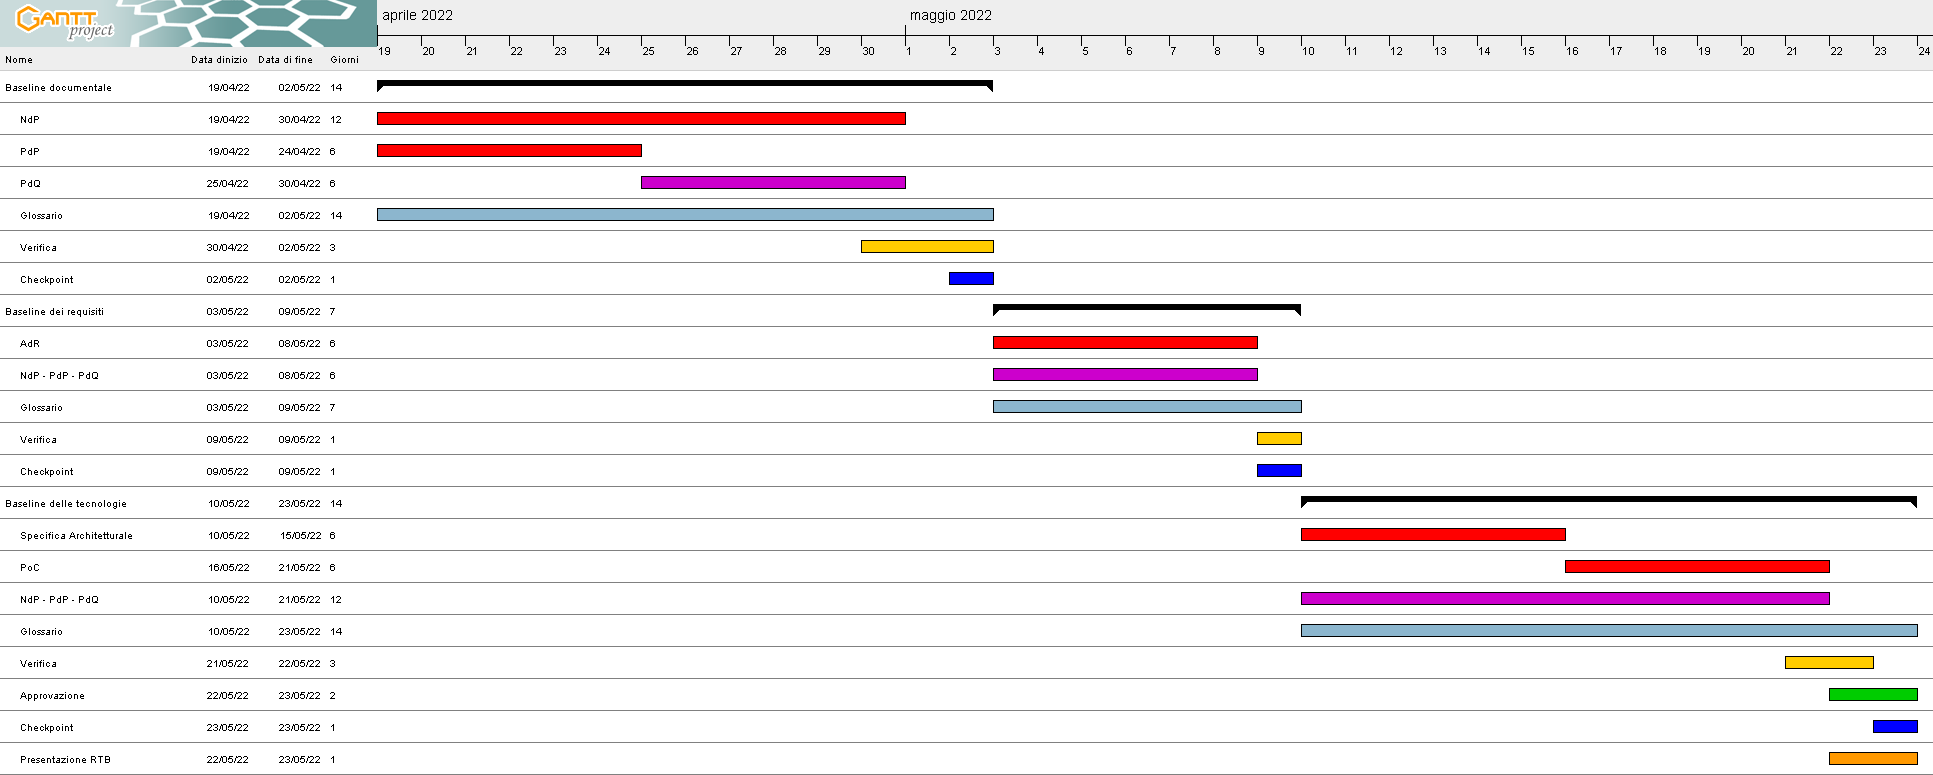
\includegraphics[width=\linewidth]{images/preventivo/RTB-Gantt.png}
    \caption{Diagramma di Gantt - Macrofase RTB}
	\end{figure}
\end{landscape}
\section{Preventivo}
      In questa sezione si riportano i preventivi per le varie fasi di lavoro elencate nel capitolo precedente. \newline
Si ricorda che il progetto didattico impone il vincolo che tutti i membri del gruppo ricoprino tutti i ruoli in modo equo.
Il gruppo rispetterà il vincolo nel progetto complessivo e non nelle singole fasi, 
altrimenti non si riuscirà a dare continuità al ruolo terminando i task assegnati.

\subsection{RTB}
\subsubsection{Baseline documentale}
\paragraph{Prospetto orario}
\begin{center}
	\renewcommand{\arraystretch}{1.8} %aumento ampiezza righe
	\begin{tabular}{ |m{10em}|c|c|c|c|c|c|c| }
	\hline
	\textbf{Membro} & \textbf{Re} & \textbf{Am} &  \textbf{An} &  \textbf{Pt} &  \textbf{Pg} &  \textbf{Ve} &  \textbf{Totale}\\
    \hline
    Irene Benetazzo   & 3 & - & 3 & - & - & - & \textbf{6} \\
    \hline
    Tommaso Berlaffa  & - & 5 & - & - & - & 1 & \textbf{6} \\
    \hline
    Mattia Episcopo   & - & 6 & - & - & - & - & \textbf{6} \\
    \hline
    Pietro Macrì      & - & 5 & - & - & - & 2 & \textbf{7} \\
    \hline
    Qi Fan Andrea Pan & - & 4 & 3 & - & - & - & \textbf{7} \\
    \hline
    Matteo Pillon     & - & 7 & - & - & - & - & \textbf{7} \\
    \hline
    Samuele Rizzato   & - & 4 & 3 & - & - & - & \textbf{7} \\
    \hline
    \textbf{Totale ore} & \textbf{3} & \textbf{31} &  \textbf{9} &  \textbf{0} &  \textbf{0} &  \textbf{3} &  \textbf{46}\\
    \hline
	\end{tabular}
\end{center}
\begin{figure}[H]
    \centering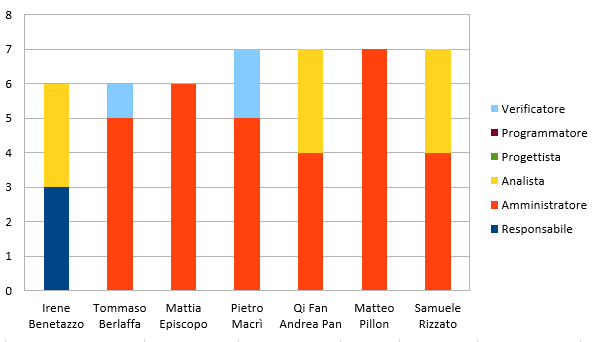
\includegraphics[width=\textwidth, height=\textheight, keepaspectratio]{images/preventivo/RTB-documentale-ore.png}
    \caption{RTB-Baseline documentale - preventivo ripartizione oraria}
\end{figure}


\paragraph{Prospetto economico}
\begin{center}
	\renewcommand{\arraystretch}{1.8} %aumento ampiezza righe
	\begin{tabular}{ |m{10em}|c|c|c|c|c|c|c| }
	\hline
	\textbf{Ruolo} & \textbf{Re} & \textbf{Am} &  \textbf{An} &  \textbf{Pt} &  \textbf{Pg} &  \textbf{Ve} &  \textbf{Totale}\\
    \hline
    Totale ore & 3 & 31 & 9 & 0 & 0 & 3 & \textbf{46}\\
    \hline
    Costo \euro/h & 30\euro/h & 20\euro/h & 25\euro/h & 25\euro/h & 15\euro/h & 15\euro/h & \\
    \hline
    \textbf{Totale costo} & \textbf{90\euro} & \textbf{620\euro} &  \textbf{225\euro} &  \textbf{0\euro} &  \textbf{0\euro} &  \textbf{45\euro} &  \textbf{980\euro}\\
    \hline
	\end{tabular}

    \begin{figure}[H]
        \centering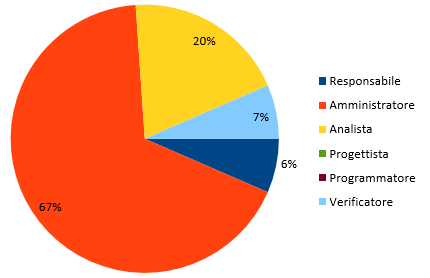
\includegraphics[width=0.7\textwidth, height=0.7\textheight, keepaspectratio]{images/preventivo/RTB-documentale-costo.png}
        \caption{RTB-Baseline documentale - preventivo ripartizione economica}
    \end{figure}
\end{center}


\subsubsection{Baseline dei requisiti}
\paragraph{Prospetto orario}
\begin{center}
	\renewcommand{\arraystretch}{1.8} %aumento ampiezza righe
	\begin{tabular}{ |m{10em}|c|c|c|c|c|c|c| }
	\hline
	\textbf{Membro} & \textbf{Re} & \textbf{Am} &  \textbf{An} &  \textbf{Pt} &  \textbf{Pg} &  \textbf{Ve} &  \textbf{Totale}\\
    \hline
    Irene Benetazzo   & - & 3 & 11 & - & - & 2 & \textbf{16} \\
    \hline
    Tommaso Berlaffa  & - & 1 & 13 & - & - & - & \textbf{14} \\
    \hline
    Mattia Episcopo   & - & 2 & 11 & - & - & - & \textbf{13} \\
    \hline
    Pietro Macrì      & - & 1 & 13 & - & - & - & \textbf{14} \\
    \hline
    Qi Fan Andrea Pan & - & 1 & 12 & - & - & - & \textbf{13} \\
    \hline
    Matteo Pillon     & - & 1 & 13 & - & - & 2 & \textbf{16} \\
    \hline
    Samuele Rizzato   & 3 & 1 & 11 & - & - & - & \textbf{15} \\
    \hline
    \textbf{Totale ore} & \textbf{3} & \textbf{10} &  \textbf{84} &  \textbf{0} &  \textbf{0} &  \textbf{4} &  \textbf{101}\\
    \hline
	\end{tabular}
\end{center}
\begin{figure}[H]
    \centering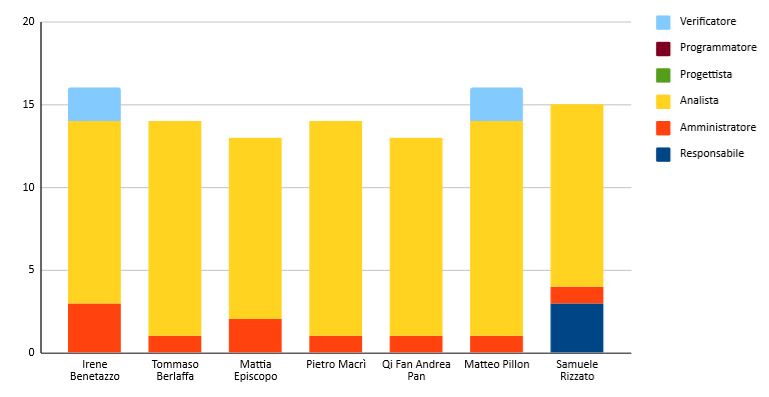
\includegraphics[width=\textwidth, height=\textheight,keepaspectratio]{images/preventivo/RTB-requisiti-ore.png}
    \caption{RTB-Baseline dei requisiti - preventivo ripartizione oraria}
\end{figure}

\paragraph{Prospetto economico}
\begin{center}
	\renewcommand{\arraystretch}{1.8} %aumento ampiezza righe
	\begin{tabular}{ |m{10em}|c|c|c|c|c|c|c| }
	\hline
	\textbf{Ruolo} & \textbf{Re} & \textbf{Am} &  \textbf{An} &  \textbf{Pt} &  \textbf{Pg} &  \textbf{Ve} &  \textbf{Totale}\\
    \hline
    Totale ore & 3 & 10 & 84 & 0 & 0 & 4 & \textbf{101}\\
    \hline
    Costo \euro/h & 30\euro/h & 20\euro/h & 25\euro/h & 25\euro/h & 15\euro/h & 15\euro/h & \\
    \hline
    \textbf{Totale costo} & \textbf{90\euro} & \textbf{200\euro} &  \textbf{2100\euro} &  \textbf{0\euro} &  \textbf{0\euro} &  \textbf{60\euro} &  \textbf{2450\euro}\\
    \hline
	\end{tabular}

    \begin{figure}[H]
        \centering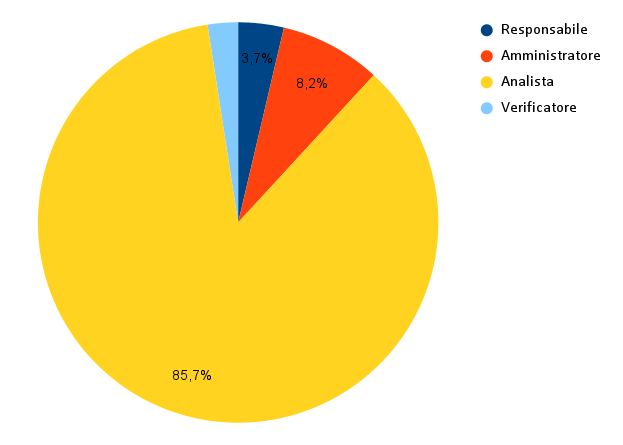
\includegraphics[width=0.7\textwidth, height=0.7\textheight, keepaspectratio]{images/preventivo/RTB-requisiti-costo.png}
        \caption{RTB-Baseline dei requisiti - preventivo ripartizione economica}
    \end{figure}
    
\end{center}

\subsubsection{Baseline delle tecnologie}
\paragraph{Prospetto orario}
\begin{center}
	\renewcommand{\arraystretch}{1.8} %aumento ampiezza righe
	\begin{tabular}{ |m{10em}|c|c|c|c|c|c|c| }
	\hline
	\textbf{Membro} & \textbf{Re} & \textbf{Am} &  \textbf{An} &  \textbf{Pt} &  \textbf{Pg} &  \textbf{Ve} &  \textbf{Totale}\\
    \hline
    Irene Benetazzo   & - & 8 & - & - & 2 & 2 & \textbf{12} \\
    \hline
    Tommaso Berlaffa  & - & - & - & 7 & 3 & 2 & \textbf{12} \\
    \hline
    Mattia Episcopo   & 1 & - & - & 8 & 3 & - & \textbf{12} \\
    \hline
    Pietro Macrì      & 1 & 1 & - & 7 & 3 & 0 & \textbf{12} \\
    \hline
    Qi Fan Andrea Pan & 3 & 2 & - & 4 & 3 & - & \textbf{12} \\
    \hline
    Matteo Pillon     & - & - & - & 7 & 3 & 2 & \textbf{12} \\
    \hline
    Samuele Rizzato   & 1 & 5 & 2 & - & 2 & 2 & \textbf{12} \\
    \hline
    \textbf{Totale ore} & \textbf{6} & \textbf{16} &  \textbf{2} &  \textbf{33} &  \textbf{19} &  \textbf{8} &  \textbf{84}\\
    \hline
	\end{tabular}
\end{center}
\begin{figure}[H]
    \centering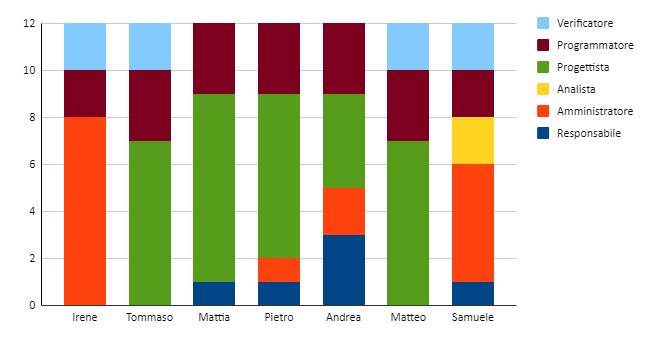
\includegraphics[width=\textwidth, height=\textheight,keepaspectratio]{images/preventivo/RTB-tecnologico-ore.png}
    \caption{RTB-Baseline delle tecnologie - preventivo ripartizione oraria}
\end{figure}

\paragraph{Prospetto economico}
\begin{center}
	\renewcommand{\arraystretch}{1.8} %aumento ampiezza righe
	\begin{tabular}{ |m{10em}|c|c|c|c|c|c|c| }
	\hline
	\textbf{Ruolo} & \textbf{Re} & \textbf{Am} &  \textbf{An} &  \textbf{Pt} &  \textbf{Pg} &  \textbf{Ve} &  \textbf{Totale}\\
    \hline
    Totale ore & 6 & 16 & 2 & 33 & 19 & 8 & \textbf{84}\\
    \hline
    Costo \euro/h & 30\euro/h & 20\euro/h & 25\euro/h & 25\euro/h & 15\euro/h & 15\euro/h & \\
    \hline
    \textbf{Totale costo} & \textbf{180\euro} & \textbf{320\euro} &  \textbf{50\euro} &  \textbf{825\euro} &  \textbf{285\euro} &  \textbf{120\euro} &  \textbf{1780\euro}\\
    \hline
	\end{tabular}

    \begin{figure}[H]
        \centering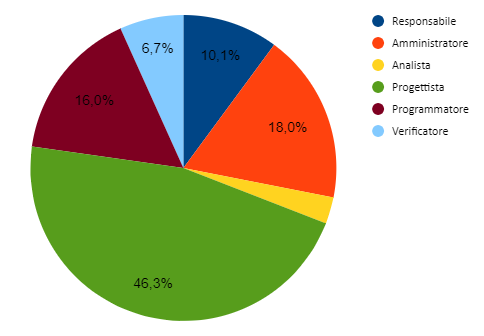
\includegraphics[width=0.7\textwidth, height=0.7\textheight, keepaspectratio]{images/preventivo/RTB-tecnologico-costo.png}
        \caption{RTB-Baseline delle tecnologie - preventivo ripartizione economica}
    \end{figure}
    
\end{center}

\newpage
\section{Consuntivo}
\end{document}